\par
\onecolumngrid
\medskip
\noindent\begin{minipage}{\textwidth}
  \centering
  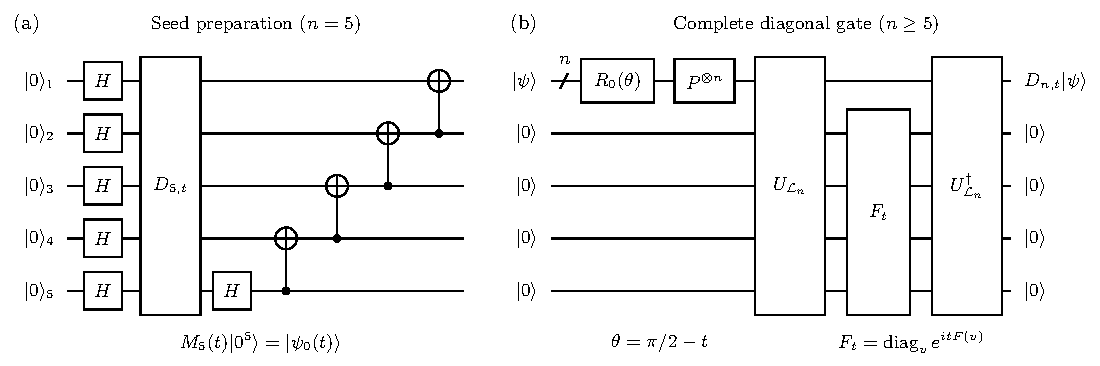
\includegraphics[width=\textwidth]{figures/fig4_clifford.pdf}
  \captionof{figure}{Circuit structure of the measurement unitary. Gates act from left to right.
  (a) Five-qubit seed preparation in the normal form of Ref.~\cite{PauwelsGisin2026}.
  (b) Decomposition of $D_{n,t}$ for every $n\ge5$, with the global phase $-i$ omitted.
  The top wire carries the $n$ data qubits, $P=\operatorname{diag}(1,i)$, and $R_0(\theta)=\exp(i\theta|0^n\rangle\langle0^n|)$ with $\theta=\pi/2-t$.
  $R_0$ is shown as an undecomposed $n$-qubit gate. Its implementation uses one clean ancilla; any of the four auxiliaries, still in $|0\rangle$ at that stage, can serve this role.
  The parity encoding $U_{\mathcal L_n}:|z\rangle|a\rangle\mapsto|z\rangle|a\oplus\mathcal L_nz\rangle$, the four-qubit gate $F_t$, and the inverse encoding implement $e^{itq_n}$ and restore the auxiliaries to $|0\rangle$.
  At $t=0$, $F_t=I$ and the encoding cancels with its inverse; $R_0(\pi/2)$ is the $X$-conjugated multi-controlled $P$ gate, recovering the decomposition of Ref.~\cite{PauwelsGisin2026}.
  At $t=\pi/2$, $R_0=I$.}
  \label{fig:clifford}
\end{minipage}
\par\medskip
\twocolumngrid
